\section{Function Points: size estimation}
\subsection{Overview}
We use the Function Points approach to estimate the size of the project. This approach makes an estimation of the size of the project based on the functionalities of system. In particular it analyses:
\begin{itemize}
\item Data structures. These can be of two types:
	\begin{itemize}[label={-}]
	\item Internal Logic Files, that are logically related data which are used and managed by the application.
	\item External Interface Files, that are logically related data which are used by the application, but are generated, reside and are managed in other applications.
	\end{itemize}
\item External Input operations, that are operations that elaborate data coming from external systems
\item External Output operations, that are operations that generate data to send to external systems .
\item External Inquiries, that are operations that involve both input and output and allow to retrieve data from Internal Logic Files and External.
\end{itemize} 
To each element of those types a weight is given, based on the complexity of the table.\newline
Multiplying the elements by their weights and summing the results we obtain the overall Function Points:\newline

\begin{equation}
FP = \sum_{}{}{Number\hspace{0.1 cm} of\hspace{0.1 cm} elements\hspace{0.1 cm} of\hspace{0.1 cm} a\hspace{0.1 cm} type * weight} 
\end{equation}

At the end, using the number of FPs, an estimation of the LOC of the project is estimated with the following formula:
\begin{equation}
LOC = AVC * number\hspace{0.1 cm} of\hspace{0.1 cm} function\hspace{0.1 cm} points
\end{equation}

AVC is a parameter that depends on the programming language used. We have chosen to use the Average value for Java among the values of the table that can be found in \cite{AVCTable}, because Java is the main language used in the project. 

\begin{figure}[h]
	\centering
	\subfigure[FP Counting Weights]{\label{fig:fp_counting}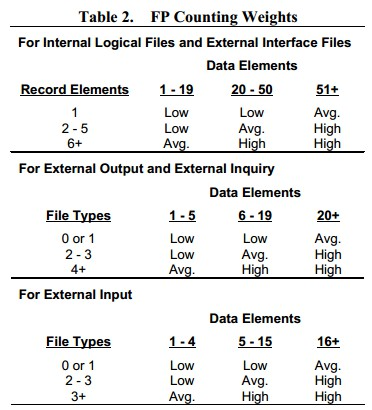
\includegraphics[width=60mm]{img/fpcounting.jpg}}
	\subfigure[UFP Complexity Weights]{\label{fig:fp_total}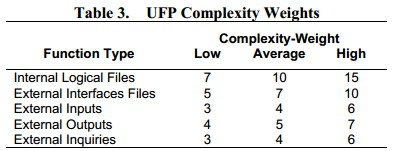
\includegraphics[width=60mm]{img/fptotal.jpg}}
	\caption{FP Analysis}
\end{figure}
\FloatBarrier


\subsection{Internal Logic Files} 

The PowerEnjoy Service needs to store information about:

\begin{itemize}
	\item \textbf{User:} This data consist in a small set of user information, for this reason its complexity has been considered \textbf{Simple}
	\item \textbf{Car:} This data consist in a small set of car information, for this reason its complexity has been considered \textbf{Simple}
	\item \textbf{Safe Area:} This data consist in a small set of safe area information, for this reason its complexity has been considered \textbf{Simple}
	\item \textbf{Trip:} This data consist in a small set of trip information, for this reason its complexity has been considered \textbf{Simple}
\end{itemize}
\fptable{			
	\fprow{User}{0}{7}	
	\fprow{Car}{0}{7}	
	\fprow{Safe Area}{0}{7}
	\fprow{Trip}{0}{7}
}

\subsection{External Interfaces File} 

\begin{itemize}
	\item \textbf{GPS positioning:} This data consist on information received by user or by OnBoard device of the car. \\Because of the managing involve some algorithms it's considered \textbf{High}
\end{itemize}

\fptable{			
	\fprow{GPS positioning}{2}{10}	
}

\subsection{External Input} 
\begin{itemize}
	\item \textbf{Sign-Up:} Create a new user entry in the system Database. \\The complexity has been considered \textbf{Simple}
	\item \textbf{Log-In/Log-Out:} Manage the user authentication. Require a module to generate an auth token\\The complexity has been considered \textbf{Medium}
	\item \textbf{Update user information:} Update users information in the system Database. \\The complexity has been considered \textbf{Simple}
	\item \textbf{Request car reservation:} Manage the car reservation in the system. Require many check on the availability.  \\The complexity has been considered \textbf{Medium}
	\item \textbf{Unlock car:} Check if the user is nearby the reserved car and send an unlock request to the car. Require algorithm on user position.  \\The complexity has been considered \textbf{Complex}
\end{itemize}

\fptable{			
\fprow{Sign-Up}{0}{3}	
\fprow{Log-In/Log-Out}{1}{4}	
\fprow{Update user information}{0}{3}	
\fprow{Request car reservation}{1}{4}	
\fprow{Unlock car}{2}{6}
}

\subsection{External Inquiries} 
A PowerEnJoy user can ask the system for the retrieval of some data:
\begin{itemize}
\item \textbf{Car list:} User can request the list of cars available in a certain area or address. Involve Geolocalization algorithms.  \\The complexity has been considered \textbf{Medium}
\item  \textbf{Special Parking Area request:} User can request the list of available special parking areas. Require to query the status of the nearby special parking area.\\The complexity has been considered \textbf{Medium}
\item  \textbf{Parking Area request:} User can request the list of parking areas. Require to query the status of the nearby special parking area. \\The complexity has been considered \textbf{Medium}
\item  \textbf{Personal Data request:} User can request to see its personal data. Data can be obtained with a simple Database Query. \\The complexity has been considered \textbf{Simple}
\item  \textbf{Trip list:} User can request the list of trips done in a certain period.\\
The complexity has been considered \textbf{Complex}
\end{itemize}

\fptable{			
	\fprow{Car list}{1}{4}
	\fprow{Special Parking Area request}{1}{4}
	\fprow{Parking Area request}{1}{4}
	\fprow{Personal Data request}{0}{3}
	\fprow{Trip list}{2}{6}
}

\subsection{External Output} 
Beyond answers to External Inquiries, the system has to send other types of messages to the user:
\begin{itemize}
\item \textbf{Reservation confirmation:} A notification of the confirmation of a reservation. Require email or push notification system. \\The complexity has been considered \textbf{Simple}
\item \textbf{End Trip notification:} A notification of the end of a trip. Require the status of the car through the OnBoard device \\The complexity has been considered \textbf{Medium}
\item \textbf{Payment notification:} A notification of the confirmation of the payment. Require an integration with the payment system \\The complexity has been considered \textbf{Medium}
\end{itemize}

\fptable{			
	\fprow{Reservation confirmation}{0}{4}
	\fprow{End Trip notification}{1}{5}
	\fprow{Payment notification}{1}{5}
}

\subsection{Results} 
According to the element in each section and their weight in complexity the total of the UFP (Unadjusted Function Points) that provide an indication of the size of the system in functional terms:

\begin{equation}
FP=ILF+EIF+EI+EQ+EO 
\end{equation}

Total Function Points: \textbf{\arabic{total_fp}}


Using 46 as AVC the final value of the estimated line of code is:

\begin{equation}
LOC = 46 * 93 = 4278
\end{equation}
